\documentclass[10pt]{article}
\usepackage{fullpage, amsfonts, amsmath, amstext, amsbsy, euscript, enumerate, amssymb, gensy
mb, wrapfig, lscape, color, graphicx, titlesec}

%TO DO LIST
%Add correlation coefficients as metric for fit in results section


\begin{document}
\pagestyle{empty}
\vspace*{2 in}
\centerline{\textbf{\LARGE Prediction of Fermentation Yields Using}}
\vspace{.25in}
\centerline{\textbf{\LARGE Artificial Neural Networks}}
\vspace{.25 in}
\centerline{\textbf{by John Abel, Kimberly Stachenfeld, Jay Stotsky, and Earl St. Sauver}}
\vspace{.125 in}
\centerline{\textbf{15 November 2012}}
\vspace{.125 in}
\centerline{\textbf{ChBE 160}}
\vspace{1 in}

\pagebreak
\section{Introduction}
%1. What are artificial neural networks? Why are they used?
Artificial Neural Networks are models that represent a relationship between inputs and outputs using a connection-based method to calculate the output. They are incredibly useful for their ability to A) concisely represent complex functions, and B) model nonlinear networks. They are typically used to model systems in a "Black Box" approach where knowledge of the underlying dynamics is relatively minimal but empirical data of the input-output relationship is readily available. The model’s structure, a weighted graph coupled with activation functions, makes tailoring the model to the empirical data provided both straightforward and computationally simple. 

%2. Why use them to model fermentation - ie: what makes fermentation tricky to model
Neural networks are often employed in cell growth models, as they provide an interface between on-line monitoring of secondary variables, and parameters of cell growth and metabolism. On-line variables such as dissolved oxygen concentration, feed rate, and volume can be measured either continuously, or frequently enough to provide a discrete model that sufficiently approximates the continuous system. The novelty of neural networks is that they can be used to create complete models for substrate concentration, metabolite concentrations (such as in the production of ethanol by fermentation) and cell concentration. 

Constructing an accurate neural model can be broken into two parts, designing the network architecture and training the network. 

The architecture of the network describes the number of internal nodes and biases, the selection of activation functions, and the use of delays and feedback loops to model the network. Multiple methods for the selection of internal network structure exist, both heuristic and empirical. A large number of guidelines, that in many ways resemble artistic rules, exist to guide the construction of the network. However these rules are both incredibly context dependent, largely are dependent on experience, and are often poorly described in the literature. A second set of techniques are based on adapting the network in the training or using a genetic algorithm to change the neural network modeling. This results in a network architecture that is individually suited to the problem, often at the expense of some computational time and obfuscation of the role of parts of the networks.

After the architecture of the network has been determined it is necessary to adapt the model to the empirical values of the system. This is done by “teaching” the network how to weight each input. The teaching involves feeding a set of inputs with known outputs, and varying weights to determine a best fit, in this case via genetic algorithm. The neural network retains these weights, and processes future data sets using these parameters, predicting behavior of complex nonlinear cell growth and production with a mathematical model.

In theory the application of a similar model in an industrial setting would be beneficial, as a finely-tuned neural network could predict cell growth and metabolism accurately without culture disruption. Currently, methods such as protein assays are used to monitor growth of a culture. However, these models are slow and labor-intensive, and do not provide real-time feedback. Neural networks are data-driven and predictive, and as such, are optimal for bioprocess monitoring, leading to savings in time and resources.

\section{Structure of Model}
\label{sec:model}

\subsection{Neural Network Model}
An artificial neural network consists of a connected system of nodes joined by weighted paths. The input to each node is weighted, and at each node, an activation function is applied. The model parameters are fed as inputs to the first layer of nodes. The outputs of this first layer are weighted and distributed to a hidden layer of eight nodes and a bias, which produce the output.

\begin{figure} %figure done with yed
\centering
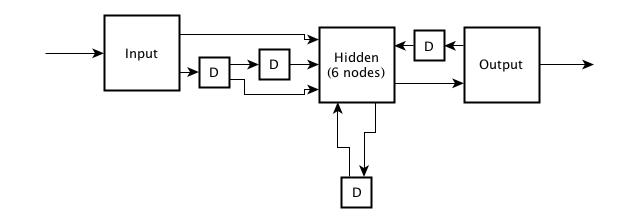
\includegraphics[scale = .5]{network_graph_ryder.jpg}
\caption{The graph above shows the system of connected nodes that make up our neural network. Each directed connected path has an associated weight. ``D’’ represents a time delay, and the value passed on will the value returned at the previous time point (two consecutive D’s refer to a double time delay, and the value will be that returned two time points ago).}
\end{figure}

\subsection{Nodes}

We use the sigmoidal activation function $f(x) = \frac{1}{1+\exp(-z)}$ at each of our nodes. The input layer consists of $19=3+3+3+6+3+1$ nodes: one node for each of the input parameters $F$, $V$ and $DO$ (3), one time-delayed node per input parameter (3), one twice-delayed node per input parameter (3), one time-delayed feedback node for each of the six nodes on the hidden layer (6), one time-delayed node per outputs $E$, $X$, and $S$ (3), and one bias (1). 

The outputs of the input layer are weighted and distributed to the six nodes of the hidden layer. The outputs of the hidden layer are again weighted, and the activation function is applied at the output level to return the predicted values of $E$, $X$, and $S$. The activation function  for the output layer is linear instead of inverse exponential.

\subsection{Estimation of Weights}

A genetic algorithm is used to select the weights for the artificial neural network. The weights on each layer are arranged as a vector, and the evaluation function calculates the sum of the difference between the E, X, and S values calculated by the neural network and those provided in the training set (the error). The evaluation function then returns the larger of two values: the inverse of the error squared, and the inverse of the absolute value of the error. The former improves resolution on the range $(0,1)$, and the latter improves resolution on $(1, \infty)$. In either case, smaller error results in larger output, and the genetic algorithm is set to favor maximum evaluation function outputs. Thus, error for all training sets should be minimized by the end of the training period.

\[ f_\text{eval}(w) = \max \begin{array}{c}\left(\frac{1}{|\Delta E|^2+|\Delta X|^2+|\Delta S|^2} , \frac{1}{|\Delta E|+|\Delta X|+|\Delta S|}\right)\end{array} \]

The weights were limited to the range -5 to 5 by default for non-delayed connections. Time-delayed signals were limited to the -1 to 1 range, since we want predictions to be based primarily on parameters with slight tweaking based 

\subsection{Training Set}
By solving the cell growth differential equation set, a comprehensive data set of inputs and outputs can be generated for training and tuning of the neural network. These training sets were created with varying feed rates so as to create a model applicable to a wide range of fermentation fed batch conditions.
The final set of training data that was found to create a very passable data set for most contexts was a random gaussian distribution between 500 and 900 for the feed.

The training set and test set feed vectors were generated by random values between 0 - 5500. Thus, the range of the feed vectors on which the model is trained would be comparable to the range given in practice.

%\subsection{Delay Paths}

Z. Chen \cite{yeastmodel} has found that there are substantial benefits to adding delays to the model. Delays allow both for some internal model correction of errors and also for the neural network training to have more coupled relationships between the inputs and outputs. The perhaps more compelling justification for the use of delays is the often notable decrease in error associated with adding delays to the process. 
In our model there are 3 separate types of delays. There are delays on the input parameters of 1 and 2 time steps. There is also a feedback from the hidden layer nodes and a feedback from the output layer. 

\section{Results}
%concentration of metabolites and stuff
%comparison of predicted to actual cell concentration and ethanol concentration
\begin{figure}[h!]
\centering
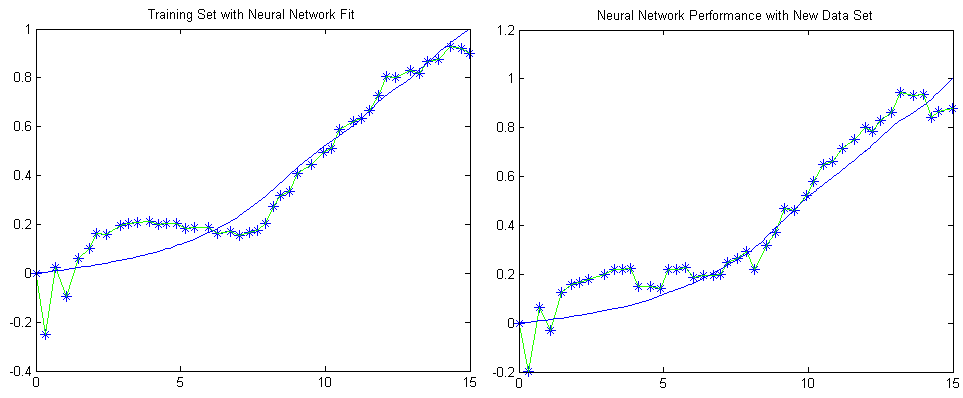
\includegraphics[scale = .3]{X.png}
\caption{Predicted and actual cell mass concentration for training set data and unfamiliar data set.}
\end{figure}
\begin{figure} [h!]
\centering
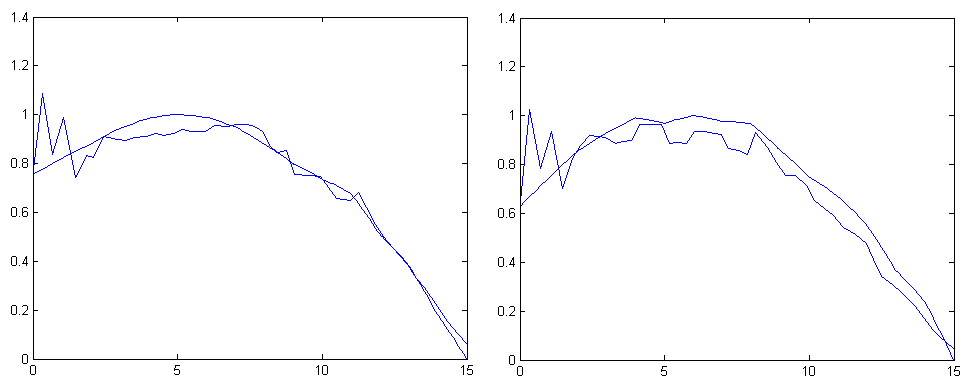
\includegraphics[scale = .3]{S.png}
\caption{Predicted and actual substrate concentration for training set data and unfamiliar data set.}
\end{figure}
\begin{figure} [h!]
\centering
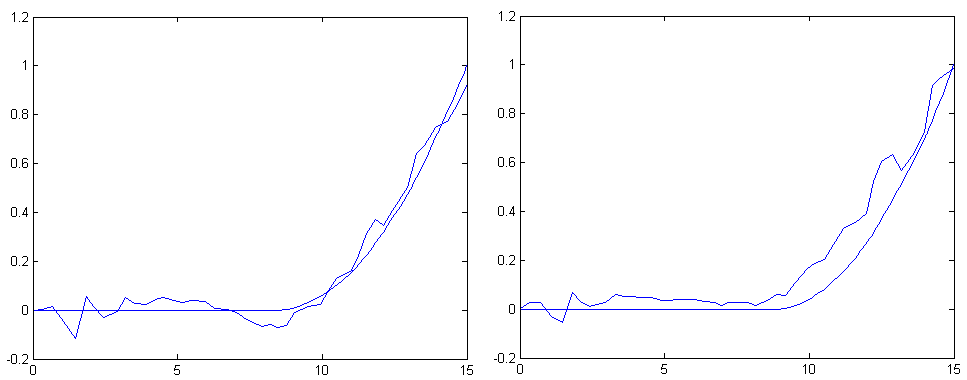
\includegraphics[scale = .3]{E.png}
\caption{Predicted and actual ethanol concentration for training set data and unfamiliar data set.}
\end{figure}

The ANN model fits the data in the training set well, indicating good recall. The slight oscillations in the error between the predicted and actual data likely could be due to random error. This is addressed in Section 4. As expected, the error between predicted and actual values is greater for the unfamiliar data set. This too is discussed in greater detail in Section 4. 

\section{Conclusions}
As shown in Figures 2, 3, and 4, the neural network provided good recall; that is, it was capable of nearly generating the training set used when fed the same input parameters. We suspect that the variability in the error between the predicted and actual concentrations are the result of edge effects in the early time points, where time-delayed values do not yet exist. 

The error was dramatically reduced when we limited the range of the weights that act on time-delayed inputs to the -1.5 to 1.5 range. Since the desired effect of these weights is to provide small adjustments to a model otherwise determined by input parameters, we wanted to confine these weights to a range of weights small relative to the size of the non-delay weights. Since the genetic algorithm is operating on a fairly large vector of weights, reducing the size of the search space greatly improved the speed, accuracy, and consistency of the model.

As expected, the model does not generalize as well as it recalled. Generalizability is improved by covering a larger range of input parameters in the training set, and this training set includes only one trial of input parameters. Thus, it is impossible for the parameters of the new data set to be included in the range covered by the training set, so the model is poorly equipped to predict metabolite concentrations given these parameters. The ANN model arrives at a nonlinear function that resembles the training set, but does not necessarily model the differential equation in general. Any degree of generalizability is likely due to functional components of the model that happen to be similar to that given by the differential equation.

%Generalizability improves when the size of the training set is increased, and increasing the number of internal nodes allows the neural network to more precisely return the exact yields given when the same parameters are used as in a member of the training set.

\section{Future Work}

\subsection{Reducing Error}
%
In general, the predicted concentrations tended to deviate most noticeably over the first few time points. This can be seen in Figures 2, 3, and 4 in Section 3. This is likely due to the absence of time-delayed inputs early on (since nothing has happened yet). The effects of these errors are seen in the slight oscillations in error seen over the rest of the signal, as the model will be constantly over-correcting for imperfect initial set of weights.

To avoid this, and to compensate for the lack of time-delay correction, we limit the acceptable error over the first few points. In effect, we are limiting our genetic algorithm initial population to a set of weights that perform adequately over the first few points. We have implemented a preliminary version of this, but plan to streamline it in the next version of the model.

\subsection{Restructuring the model}
We will want to first modify our model so that it can be trained using multiple training sets instead of just one. This will allow the network to predict 

In addition, we will experiment with the mutation options available in the genetic algorithms package to find a method optimally suited for weight determination. A mutation method that uses too large a number of the population to make the next population will be limited by the worst set among those, and a mutation that uses too few will not explore a large section of the sample space. We therefore expect to see differences in the speed and accuracy of the model by altering the mutations.

We also want to examine the effect of using different activation functions for the nodes. For instance, according to the literature, it is common to include a layer that uses a linear activation function instead of the sigmoidal. Including a greater variety of nodes should allow us to capture a more diverse range of nonlinear characteristics.

\subsection{Statistical selection of the training set}
We will want to involve the inclusion of a filtering system that evaluates how influential a certain sample set should be in the training of our model and weights it accordingly. Sets dubbed outliers will be minimally influential, and those highly representative of the sample will be more heavily weighted. The degree to which a set is an outlier will be determined by calculating a distance measure between that set and all other sets. Then sets will be ranked by their proximity to other members of the set: for instance, the average distance of the 5 closest sets to a set, or the distance to the “center of mass” of the set space. Alternatively, a Bayesian filter could be used in place of a distance metric. This analysis returns a probability that the set represents the actual process, and this probability will be used to weight the influence of that data set.


\subsection{Generalizability versus Recall}
``Recall,’’ the ability of a network to return the values given by the training set when inputted the corresponding parameters, will increase as nodes are added to the network if the size of the training set is kept constant. These extra nodes allow greater versatility in the number of signals that can be simulated, and can therefore fit a greater number of nodes more closely. However, this method is subject to overfitting, since random variations in the data set will be precisely accounted for as well. Thus, when unfamiliar parameters are inputted to the model, what were only random variations seen in the training set will result in false predictions.

Increasing the size of the data set relative to the number of nodes decreases the networks capacity for recall, but increases “generalizability,” the ability of the network to predict the outcome given unfamiliar parameters.

\begin{thebibliography}{9}

%Genetic Algorithm Items
\bibitem{hybridoma} ~~de Tremblay, ~M., et al. \emph{Optimization of fed-batch culture of hybridoma cells using dynamic programming: single and multi-feed cases.} Bioprocess Engineering, vol. 7, pp. 229-234, (1992)
\bibitem{ga} ~Houck, ~C. ~R., ~Joines, ~J.~A., and ~Kay, ~M.~G. \emph{A Genetic Algorithm for Function Optimization: A Matlab Implementation.}

\bibitem{softsens} Assis, A. J. and R. M. Filho. \emph{Soft sensors development for on-line bioreactor state estimation}. Computers and Chemical Engineering 24 (2000) 1099-1103.
\bibitem{neral} Thibault, J., V. Van Breusegem, and A. Cheruy. \emph{On-Line Prediction of Fermentation Variables Using Neural Networks} Biotechnology and Bioengineering (1990) Vol. 36, 1041-1-48.
\bibitem{yeastmodel} Chen, L. Z. et. al. \emph{Soft Sensors for on-line biomass measurements}. Bioprocess and Biosystems Engineering. (1996) Vol. 26 (3), 191-195.

\end{thebibliography}
\end{document}

